\subsubsection{Hypothesis 1: Education and Employment Status}

\begin{table}[H]
    \caption{Chi-Square Test Results}
    \label{tab:chi_square_results}
    \begin{minipage}{\columnwidth}
        \centering
        \begin{tabular}{lll}
\toprule
 & $\chi^2$ & $p$ \\
\midrule
Value & 905.29 & 0.00 \\
\bottomrule
\end{tabular}

    \end{minipage}
\end{table}

\begin{table}[H]
    \centering
    \scriptsize
    \caption{Logistic regression results}
    \begin{minipage}{\columnwidth}
        \begin{center}
\begin{tabular}{lclc}
\toprule
\textbf{Dep. Variable:}      & employ\_Status2  & \textbf{  No. Observations:  } &    28853    \\
\textbf{Model:}              &      Logit       & \textbf{  Df Residuals:      } &    28851    \\
\textbf{Method:}             &       MLE        & \textbf{  Df Model:          } &        1    \\
\textbf{Date:}               & Mon, 30 Sep 2024 & \textbf{  Pseudo R-squ.:     } &  0.01560    \\
\textbf{Time:}               &     15:55:34     & \textbf{  Log-Likelihood:    } &   -18330.   \\
\textbf{converged:}          &       True       & \textbf{  LL-Null:           } &   -18621.   \\
\textbf{Covariance Type:}    &    nonrobust     & \textbf{  LLR p-value:       } & 2.302e-128  \\
\bottomrule
\end{tabular}
\begin{tabular}{lcccccc}
                             & \textbf{coef} & \textbf{std err} & \textbf{z} & \textbf{P$> |$z$|$} & \textbf{[0.025} & \textbf{0.975]}  \\
\midrule
\textbf{const}               &       0.4097  &        0.046     &     8.951  &         0.000        &        0.320    &        0.499     \\
\textbf{education\_category} &      -0.3346  &        0.014     &   -23.366  &         0.000        &       -0.363    &       -0.307     \\
\bottomrule
\end{tabular}
%\caption{Logit Regression Results}
\end{center}
    \end{minipage}
\end{table}

\begin{figure}[H]
    \centering
    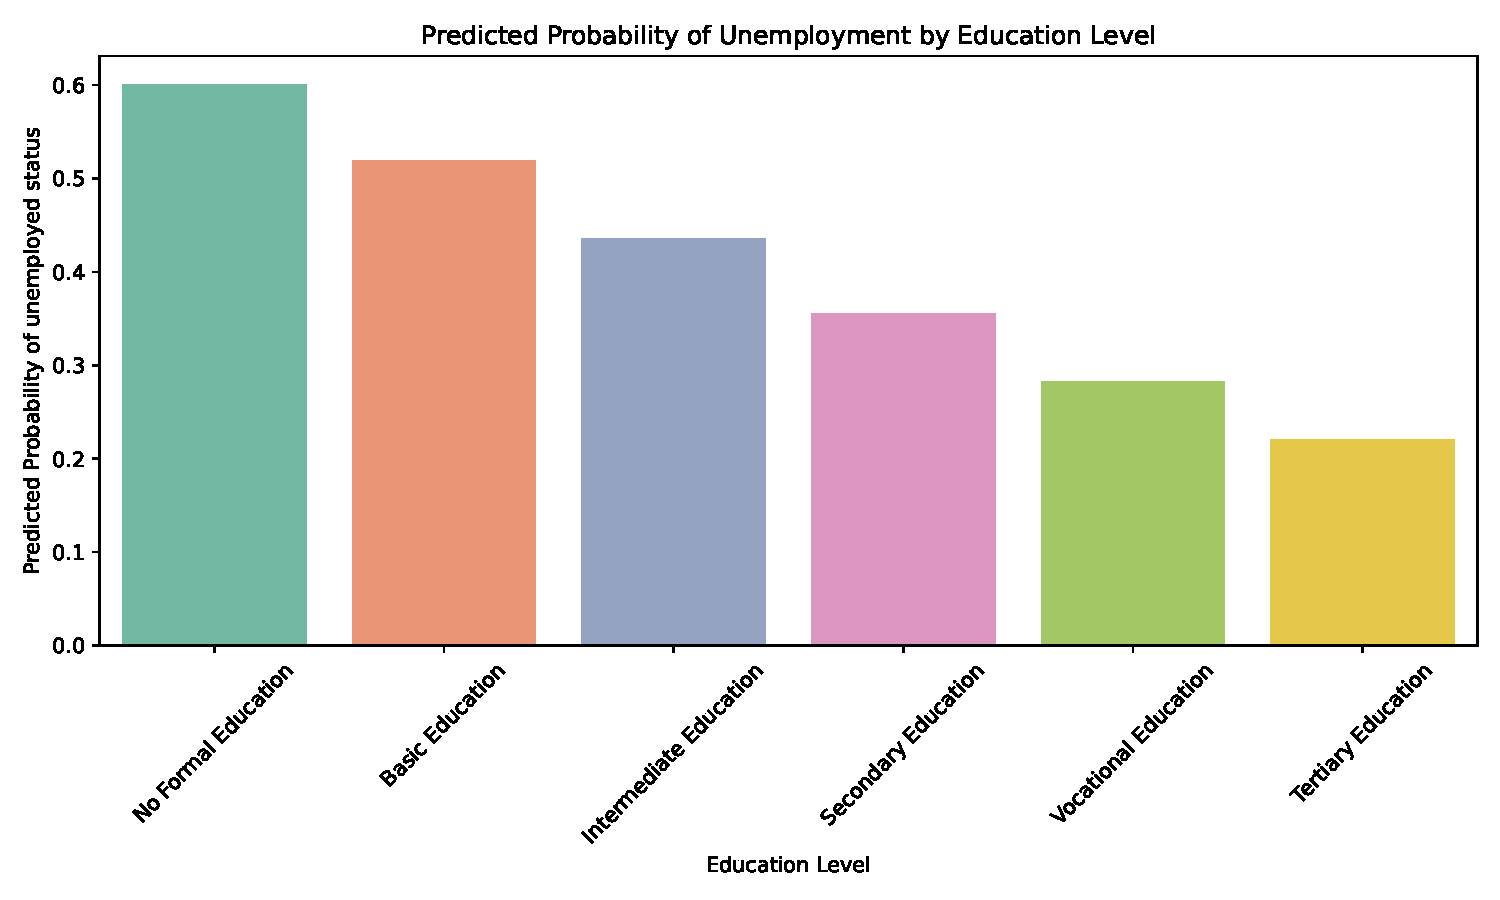
\includegraphics[width=\columnwidth]{images/hyp_1_log_pred.pdf} % Adjust the path accordingly
    \caption{Predicted probability of unemployment by Highest level of education group}
    \label{fig:predicted unemployment for highest academic level}
\end{figure}

\begin{figure}[H]
    \centering
    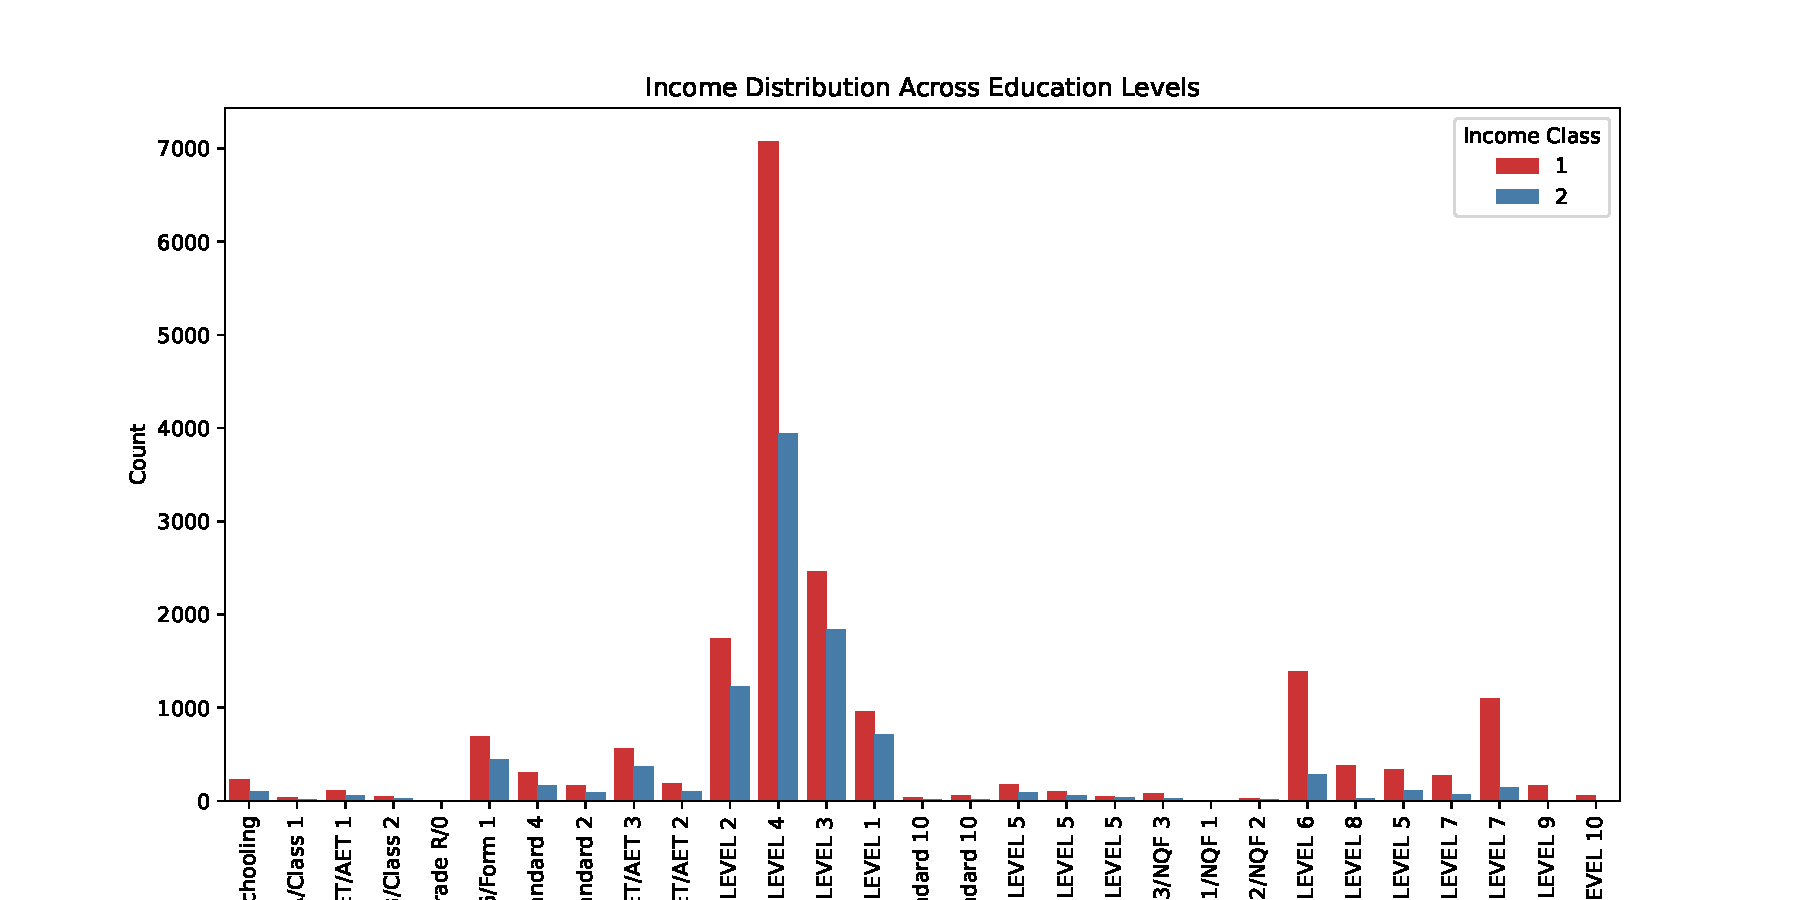
\includegraphics[width=\columnwidth]{images/hyp_1_income_dist.pdf} % Adjust the path accordingly
    \caption{Income distribution over detailed highest level of education}
    \label{fig:unemployment distribution for unemployment highest academic level}
\end{figure}

The chi-square test for independence showed a significant relationship between education level and employment status ($\chi^2 = X.XX$, $p < 0.05$). This suggests that higher levels of education are associated with higher employment rates.
